\documentclass{beamer}
\usepackage[style=authortitle-comp]{biblatex}
\usepackage[export]{adjustbox}

\title{Progress Report: Cache Replacement, Application Performance, and Relations to DSM}
\author{Zhengyi Chen} % Amir?
\date{\today}

\addbibresource{../main.bib}

\begin{document}
% Title page
\frame{\titlepage}

% Page 1
\begin{frame}
    \frametitle{(Cache) Replacement Strategies}
    \begin{itemize}
        \item There have been significant development in (CPU) cache replacement strategies in the last decades.
        \item e.g., RRIP(++)\footcite{JTSE.2010.RRIP} and more recently (various) ML-\textit{derived} heuristics.
        \item Also popular is studying adequate cache replacement strategies for distributed systems (though more stagnant).
        % There is a lack of translation between advancements in hardware and their efficacy in software.
        % That said, this might be because they are (able to afford) machine learning techniques in dynamic replacement strategies at edge nodes...
        \item There are many variables within each cached system (whether CPU or distributed FS, etc.) that affect which strategy is more \textit{efficient} in operation.
        % A cached/distributed FS or CDN, for example, primarily captures frequency than recency.
        % An operating system might juggle between both depending on the type of access -- Linux's LRU_GEN attempts to capture this difference between file descriptor
        % accesses and just plain stack/heap/text section accesses.
        % The replacement problem for our kernel DSM is similar -- we want to capture the working set of all in-scope processes for each node in system. The existence of
        % swap space only complicates the matter:
        % - Swap locally to swap file?
        % - Swap remotely to other node's memory which our DSM might be able to do?
        % - Swap remotely to other node's swap file?
        % As Amir mentioned there is also the question of speed -- the replacement algorithm needs to be fast enough for the system to not stall, though the problem
        % of selecting a replacement algorithm may not (need to) be as time-sensitive?
        \item Moreover, different applications (e.g., threads) exhibit different access patterns which may be better served by one strategy than another.\footcite{SYS.2021.RLR}
    \end{itemize}
\end{frame}

% Page 2
\begin{frame}
    \frametitle{Notable (i.e., Encountered) Strategies}
    \begin{itemize}
        \item LRU family
        \item FIFO family
        \item Adaptive Replacement Cache
        \item CPU-LLC Intended: Dynamic Insertion Policy, Re-Reference Interval Prediction, Signature-based Hit Predictor, \dots
        % RRIP is basically an M-bit LFU.
        \item ML-derived: Reinforcement Learned Replacement, LeCaR, Cache Replacement Problem as Markov Decision Process\footcite{GWHSZ.2014.CacheReplAsMDP-QLearning},
              \dots
    \end{itemize}
\end{frame}

% Page 3
\begin{frame}
    \frametitle{Notable (i.e., Encountered) Strategies}
    \begin{itemize}
        \item The performance of replacement strategies correlate strongly to the context of their operation.
        \item For example, LRU is theoretically better-performing than FIFO \textit{in their most textbook implementations} but recent studies
              \footcites{EHOFK.2020.IBM-LRUvsFIFO}{YQZYR.2023.FIFOwithTwist} have shown that FIFO can outperform LRU in practice (CDNs, for example, where even cache
              bookkeeping structures can be costly).
        % Now it's probable that these papers are unfairly competing a more state-of-the-art FIFO-esque algorithm with a less so LRU-esque algorithm...
        % In general:
        \item To summarize, \textbf{The (dynamic) choice of replacement algorithm in any system is of practical concern!}
    \end{itemize}
\end{frame}

% Page 4
\begin{frame}
    \frametitle{LRU \& FIFO family -- Patches and Applications}
    \begin{itemize}
        \item The state-of-the-art implementations of LRU or FIFO is far-cry from their textbook implementations.
              % Also there are a LOT of them -- I can't find enough time to gather all of them RN.
        \item This is so that they can capture both \emph{recency} and \emph{frequency}:
              we desire to use both to predict/assume the \emph{re-reference interval} of a given entry.
        \item e.g., Linux uses \texttt{LRU\_GEN} which is a multi-queue LRU strategy wherein each queue(generation) represents a "similar" level of access recency and is evicted in batch.
        \item The kernel developers wanted a \emph{fast and reasonably good} replacer as opposed to an optimal one.
              % optimality and performance should both be considered when selecting replacement strategies.
        \item Likewise, Yang, et.al.\footcite{YQZYR.2023.FIFOwithTwist} shows that FIFO with \textit{lazy promotion} and \textit{quick demotion} outperforms textbook LRU.
              % recall that FIFO can exploit spatial locality better than LRU particularly in systems with slow data access!
              % i.e., algorithm performance can be constrained by system topology.
    \end{itemize}
    % The documentation of LRU_GEN really shows that the developers wanted the strategy itself to decide fast (as opposed to merely deciding well): the strategy itself "[tries] to profit from spatial
    % locality"
\end{frame}

% Page 5
\begin{frame}
    \frametitle{\texttt{LRU\_GEN} and Access Patterns}
    The \texttt{LRU\_GEN} algorithm specifically makes stronger protection of pages for memory accesses through PT than through FD: \
    \begin{itemize}
    \item Heap/Stack/Text access misses have higher cost -- executables perform blocking I/O at memory access, less likely for file access.
    \item They are also more likely to miss, as their in-kernel dirty bits are approximated.
    \item Finally, they can be reasonably assumed to more likely exhibit temporal locality.
    \end{itemize}
    Nevertheless, the algorithm is capable to dynamic adjustment on re-faults -- \textbf{the data model of programs can be file-based or object-based}.
    % Though as we know files (i.e., blocks in which file data reside) are loaded into (kernel) memory and heap allocation can always be swapped out,
    % so I guess object-based storage wins with less intermediate steps (e.g., filesystem calls), sans data protection.
    The same algorithm can deviate in fault rates on different programs on the same node.
    % i.e., any good algorithm must be able to dynamically adapt to fault rate feedbacks.
    % However, we don't want to run them through any complex learner...
\end{frame}

% Page 6
\begin{frame}
    \frametitle{Machine Learning as Analytic Tool: RLR, etc.}
    \begin{itemize}
        \item Large distributed systems (e.g., CDNs) can afford to perform machine learning for cache replacement tasks
              \footcite{GWHSZ.2014.CacheReplAsMDP-QLearning}: run-time is much faster than I/O so some cycles could be afforded.
        \item For page replacement in kernel, we can't really afford to run anything costly (Amir).
        \item ML analysis\footcite{SYS.2021.RLR} shows how different (computation-intensive) programs exhibit distinct
              access patterns.
    \end{itemize}
\end{frame}

% Page 7
\begin{frame}
    \frametitle{Machine Learning as Analytic Tool: RLR, etc.}
    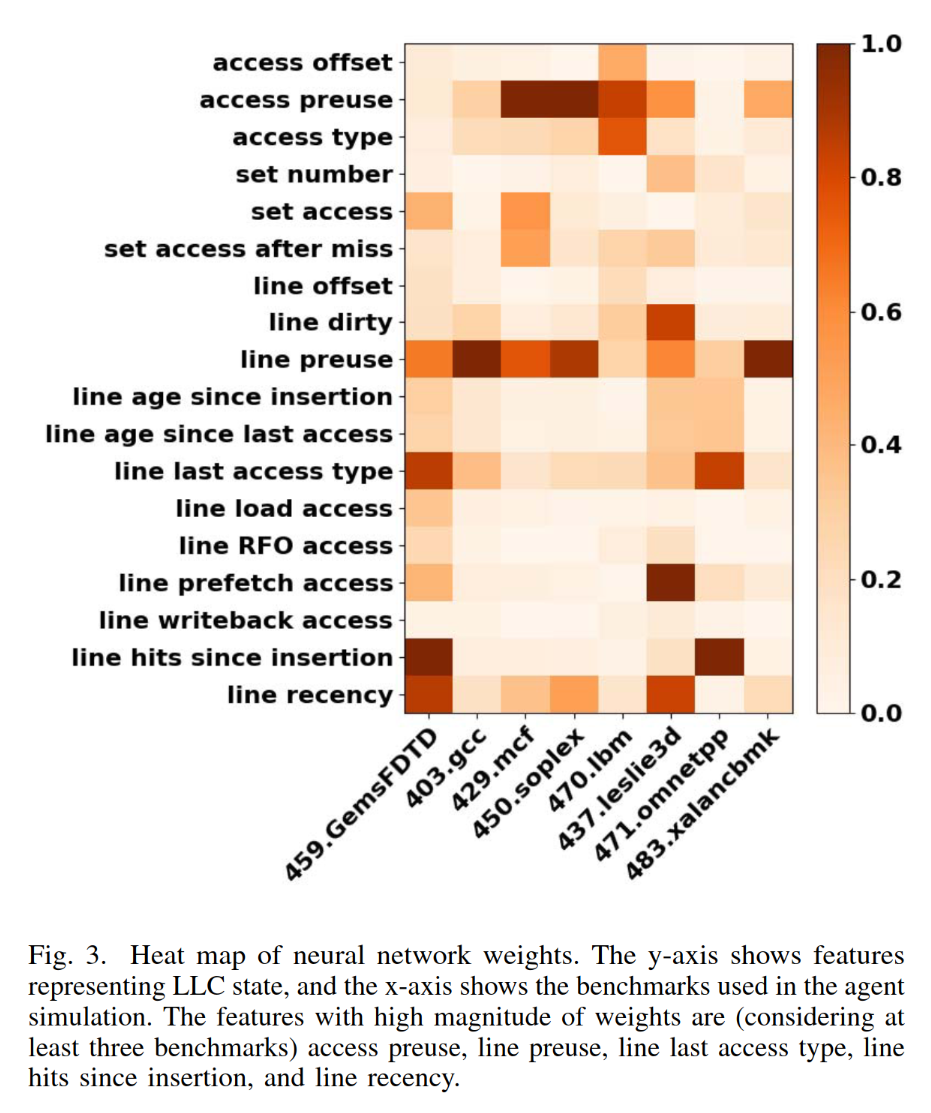
\includegraphics[height=0.6\textheight, center]{w4_slices_resources/RLR.Fig3.png}
    \footcite{SYS.2021.RLR}
    P.S. \textit{preuse}: set access since last access to address/line.
\end{frame}

% Page 8
\begin{frame}
    \frametitle{DSM, Applications, and Memory (Contention)}
    The speedup of applications on DSM systems is negatively correlated to shared memory contention.

    Take TreadMarks\footcite{CDKP.1994.TreadMarks} for example:
    \begin{itemize}
        \item \textit{Jacobi} is a solver for linear system of equations via the \textit{successive over-relaxation} method.
               The memory access pattern should be map-reduce-like: the problem is parallelized w/ partial matrices for each node with immutable storage of the relevant matrices?
               TreadMarks achieves $\sim7x$-speedup on a 8-node system over one single-core node.
        \item \textit{Water} is a parallel $N$-body molecular dynamics simulator that requires at least $O(\frac{N}{2})$ communications per processor.
               TreadMarks only achieves $\sim4x$-speedup with around $47\%$ time used for blocking communications.
    \end{itemize}
\end{frame}

% Page 9
\begin{frame}
    \frametitle{DSM, Applications, and Memory (Contention)}
    \begin{itemize}
        \item It's kinda difficult to compare statistics from different DSM systems.
        \item Even with the same programs being run, different parameters makes for different program behaviors wrt. contention, etc.
        \item Logically speaking, the more contention on the same address, the less speedup is possible for the system\footcite{de2000effect}.
        \item Should cache replacement strategies be aware of how contended a page may be to prevent it from e.g., being swapped out?
    \end{itemize}
\end{frame}

% Page 10
\begin{frame}
    \frametitle{Hardware-based Dynamic Strategy Selection: DIP}
    Hardware-based replacement strategies can provide low-cost inspirations for software replacement strategies.

    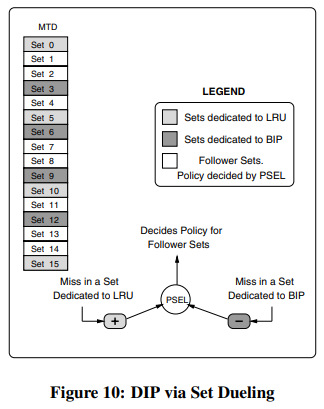
\includegraphics[height=0.6\textheight, center]{w4_slices_resources/DIP.Fig10.png}\footcite{QJPSE.2007.DIP}

    Problem: How can this be scaled for multiple strategies?
\end{frame}

\end{document}